\documentclass[hidelinks, 12pt,a4paper]{article}
\usepackage[utf8]{inputenc}
\usepackage[T1]{fontenc}
\usepackage[a4paper,left=2cm,right=2cm,top=2cm,bottom=2cm]{geometry}
\usepackage[english,francais]{babel}
\usepackage[french]{varioref}
\usepackage{libertine}
\usepackage[pdftex]{graphicx}
\usepackage{geometry}
\usepackage[pdftex]{graphicx}
\usepackage{adjustbox}
\usepackage{color}
\usepackage{setspace}
\usepackage{hyperref}
\usepackage{comment}
\usepackage{fancyhdr}
\pagestyle{fancy}

\setlength{\parindent}{0cm}
\setlength{\parskip}{1ex plus 0.5ex minus 0.2ex}
\newcommand{\hsp}{\hspace{20pt}}
\newcommand{\HRule}{\rule{\linewidth}{0.5mm}}

\renewcommand{\baselinestretch}{1.3}
\renewcommand{\headrulewidth}{1pt}
\fancyhead[L]{}
\fancyhead[C]{\textbf{Le Petit Scientifique}}
\fancyhead[R]{
\includegraphics[width=2.5cm]{images/universite-rouen.jpg}}

\begin{document}

\begin{titlepage}
  \begin{sffamily}
  \begin{center}

    % Upper part of the page. The '~' is needed because \\
    % only works if a paragraph has started.

    \textsc{\LARGE UFR des Sciences et Techniques}\\[2.5cm]

    \textsc{\Large Rapport Mini projet LW1 – sCiMS}\\[1.5cm]

    % Title
    \HRule \\[0.4cm]
    { \huge \bfseries Le Petit Scientifique\\[0.4cm] }

	\HRule \\[2cm]
    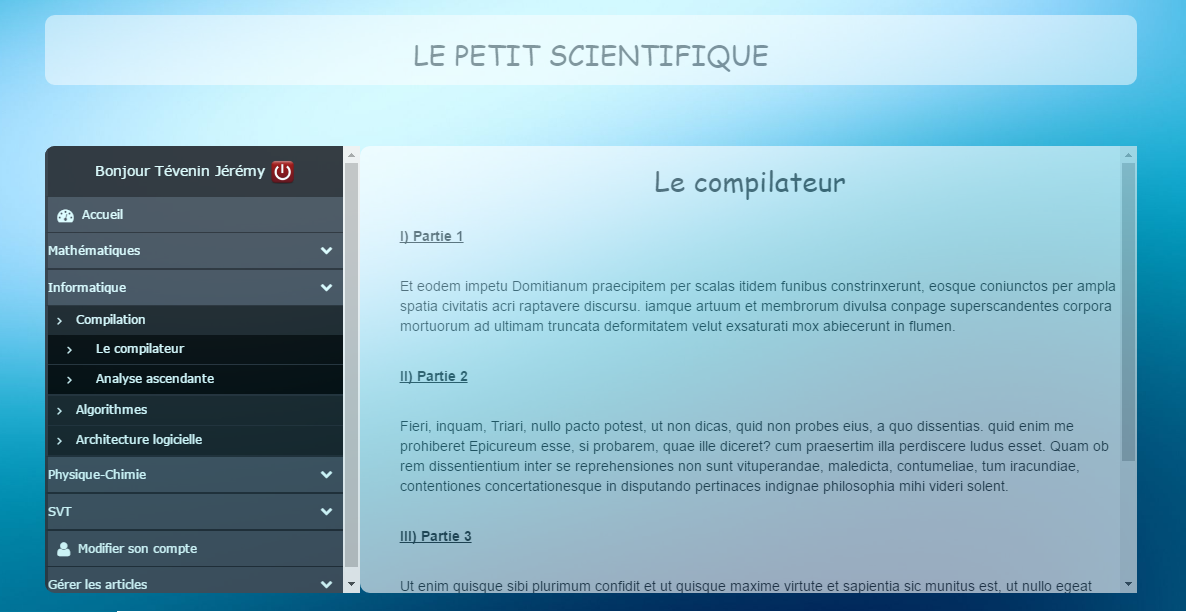
\includegraphics[scale=0.5]{images/accueil2.png}
    \\[2cm]

    % Author and supervisor
    \begin{minipage}{0.4\textwidth}
      \begin{flushleft} \large
        Amine \textsc{BOUAZIZ}\\
        Jérémy \textsc{TEVENIN}\\
      \end{flushleft}
    \end{minipage}
    \begin{minipage}{0.4\textwidth}
      \begin{flushright} \large
        \emph{Rendu à :} M. \textsc{Mallet}\\
      \end{flushright}
    \end{minipage}

    \vfill

    % Bottom of the page
    {\large 22 décembre 2016}

  \end{center}
  \end{sffamily}
\end{titlepage}

\newpage
%Table of contents
\tableofcontents

\newpage
\section{Introduction}
Le projet consiste en l'écriture d'un mini CMS pour la mise en ligne d'articles à caractère scientifique.

Le site sera divisé en catégories, sous-catégorie et articles pour organiser le contenu.
Il y a 3 types d'utilisateurs ~:\\ 
\begin{itemize}
\item l'administrateur qui peut gérer les catégories, sous-catégories et rédacteurs
\item les rédacteurs peuvent ajouter des articles et ils peuvent aussi modifier ou supprimer leur propre articles 
\item les simples utilisateurs peuvent juste visionner les articles
\end{itemize}

\newpage
\section{Manuel d'utilisation}
Pour lancer le site, nous utilisons un serveur wamp. Il suffit de placer le dossier de notre projet dans le dossier de votre serveur.\\

Nous vous fournissons des fichiers sql contenant nos deux bases de données (AUTEUR et MENU). Elles se trouvent dans le dossier ``Bases\_de\_données''.\\

Il vous suffit d'importer ces fichiers sql et de lancer index.php qui vous redirigera vers la page d'accueil.\\

Les identifiant de connexion à la base sont par défaut ``root'' et le mot de passe est vide. Si votre serveur à des identifiants différents, vous trouverez un fichier config.php où vous changerez les identifiants ``USER'' ET ``PASSWD''.\\

\begin{tabbing}
\hspace{2cm}\=\hspace{2cm}\=\kill
<?php\\
\>	define('HOSTNAME','localhost');\\
\>	define('USER','root');\\
\>	define('PASSWD','');\\
\>	define('DBMENU','menu');\\
\>	define('DBAUTEUR','auteur');\\
?>\\
\end{tabbing} 
Vous pourrez vous connectez en mode administrateur en vous connectant avec ~:\\
\begin{itemize}
\item admin@admin.fr
\item Admin0
\end{itemize}

Ou en se connectant avec un rédacteur avec ~:\\
\begin{itemize}
\item jeremy\_tevenin@hotmail.fr
\item Jeremy76\\
\end{itemize}

(Attention aux majuscules !)\\

Vous pouvez aussi créer votre propre rédacteur ou simplement lire les articles sur le site.

\newpage
\section{Conception}
Pour concevoir notre application, nous avons utiliser un modèle MVC. Notre application contient deux parties différentes ~:\\
\begin{itemize}
\item la partie accueil permettant de se connecter ou de s'inscrire
\item la partie site permettant de lire les articles ou de les administrer
\end{itemize}

Comme nous avons deux parties, nous avons deux contrôleurs différents, acceuil.php et lepetitscientifique.php.\\

Voici un schéma de notre application.\\

\begin{center}
\includegraphics[width=16cm]{images/diag.png}\\
\end{center}


Nous avons aussi un dossier images contenant les images du site, un dossier articles qui contient les articles du site.
 
\newpage
\section{Les bases de données}
\subsection{Menu}
La base de données MENU contient toutes les catégories, sous-catégories et articles.\\

Table categorie : \\
\begin{itemize}
\item id auto-incrémenté
\item nom
\end{itemize}

Table souscategorie : \\
\begin{itemize}
\item id de référence à categorie
\item id auto-incrémenté
\item nom
\end{itemize}

Table article : \\
\begin{itemize}
\item id de référence à souscategorie
\item id auteur
\item id auto-incrémenté
\item date
\item nom
\item repertoire permet de savoir où est stocké l'article
\item url permet de savoir le nom de l'article
\end{itemize}

\subsection{Auteur}

Table auteur : \\
\begin{itemize}
\item id auto-incrémenté
\item nom
\item ville
\item mail qui va permettre la connexion au site
\item un mot de passe
\item un booléen qui détermine le niveau d'administration
\end{itemize}

\newpage
\section{Inscription/connexion}
Un utilisateur peut se connecter si il a déjà un compte, s'inscrire pour devenir rédacteur ou simplement visiter le site.

\subsection{Inscription}
Pour s'inscrire sur le site, il remplir un questionnaire. Tout se passe sur la page d'accueil où l'utilisateur peut remplir ce questionnaire. \\

\begin{center}
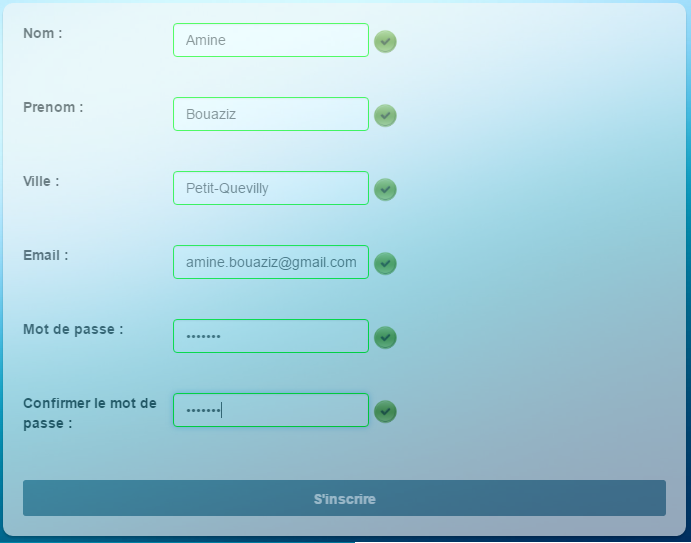
\includegraphics[scale=0.8]{images/inscriptionvalid.png} 
\end{center}

Il doit remplir tous les champs pour pourvoir envoyer le formulaire ! Tant qu'il n'a pas rempli tous les champs, le formulaire ne peut pas être envoyé Pour cela, nous avons utilisé les fonctionnalités de JQuery. Chaque input est géré par des fonctions gérant la couleur et les messages d'erreurs. C’est le fichier script.js qui gère tout cela. Il y a aussi des sécurités avec des patterns, required et des htmlspecialchar sur les valeurs reçu.
Le mot de passe est hashé avec la méthode password\_hash() avant d'être mis dans la base de données.\\


\begin{center}
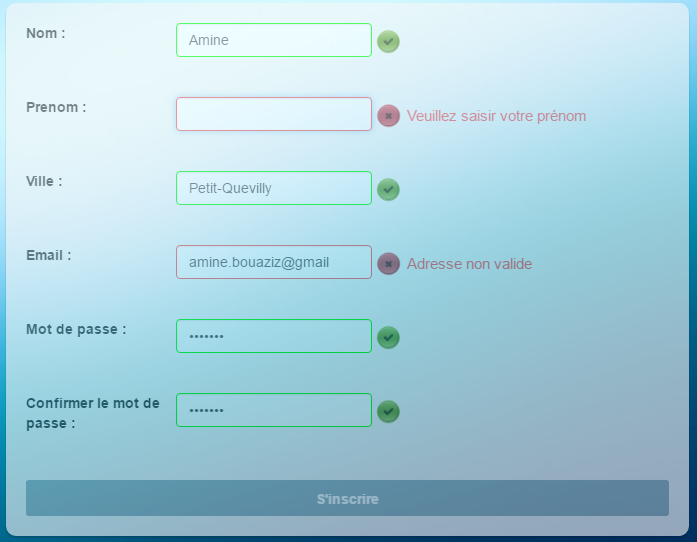
\includegraphics[scale=0.8]{images/inscriptionnnvalid.png}\\
\end{center}

Il ne peut 

\subsection{Connexion}

\newpage
\section{Administration du site}
\subsection{Par l'administrateur}
\subsubsection{Gérer les catégories}
\subsubsection{Gérer les sous-catégories}
\subsubsection{Gérer les rédacteurs}

\newpage
\subsection{Par les rédacteurs}
\subsubsection{Créer un article}
\subsubsection{Modifier un article}
\subsubsection{Supprimer un article}


\newpage
\section{Le style du site (CSS)}

\newpage
\section{Conclusion}

\end{document}
